\documentclass[letterpaper]{article}
\usepackage[utf8]{inputenc}
\usepackage{cool}
\usepackage{gensymb}
\usepackage{mathtools}
\usepackage[portuguese]{babel}
\usepackage{colonequals}
\usepackage{indentfirst}
\usepackage{commath}
\usepackage{titlesec}
\usepackage{multicol}
\usepackage{float}
\usepackage{graphicx}
\usepackage{amsmath}
\usepackage{esvect}
\usepackage{multirow}
\usepackage{longtable}
\usepackage{algorithm,algpseudocode}
\usepackage[]{algorithm2e}
\usepackage{comment}
\usepackage{amssymb}
\usepackage{xcolor}
\usepackage[inline]{enumitem}

\renewcommand{\thefootnote}{\arabic{footnote}}
\newcommand*{\logeq}{\Leftrightarrow}
\newcommand*{\logim}{\Rightarrow}
\newcommand*{\N}{\mathbb{N}}

\makeatletter
\renewcommand{\fnum@algorithm}{\fname@algorithm}
\makeatother

\usepackage{geometry}
\geometry{margin=2cm}
\setlength{\textfloatsep}{7pt plus 1.0pt minus 1.0pt}
\textheight = 650pt 
\marginparsep = 5pt
\setlength{\columnsep}{10pt}
\geometry{bottom=2.5cm}

\titleformat*{\section}{\large\bfseries}
\titleformat*{\subsection}{\small\bfseries}
\titleformat*{\subsubsection}{\small\bfseries}

\title{Implementação da Decomposição Empírica Modal e \\ Exemplos de Aplicação \vspace{5mm}\small{\\Instituto Superior Técnico\\ Mestrado Integrado em Engenharia Física Tecnológica\\Física Computacional}}
\author{Por \textbf{Ana Filipa Valente (90376)} e \textbf{Inês Alves Ferreira (90395)}}

\usepackage{fancyhdr}
\pagestyle{fancy}
\fancyhf{}
\rhead{Física Computacional}
\lhead{Implementação da Decomposição Empírica Modal e Exemplos de Aplicação}
\rfoot{\thepage}
\cfoot{MEFT 2018/2019}
\renewcommand{\headrulewidth}{2pt}
\renewcommand{\footrulewidth}{1pt}

\begin{document}

\maketitle

\noindent\rule{16cm}{0.4pt}
\begin{abstract}
\noindent

Este trabalho compreende o desenvolvimento de uma implementação em $\textsc{C}_{++}$ (com recurso à biblioteca \textsc{ROOT}) da decomposição empírica modal de um sinal temporal. O texto abaixo encontra-se dividido de tal forma que: \begin{enumerate*}[label = \textbf{(\arabic*)}] \item A Secção \ref{sec:intro} introduz o conceito de decomposição empírica modal e propõe um algoritmo para a sua computação. \item A Secção \ref{sec:implement} propõe uma implementação para o algoritmo descrito na secção anterior. \item A Secção \ref{sec:exemplos} providencia exemplos de correção do código desenvolvido. \end{enumerate*} 
\end{abstract}

\noindent\rule{16cm}{0.4pt}

\begin{multicols}{2}

\section{Introdução}
\label{sec:intro}

\par A decomposição empírica modal (abreviada por \textit{EMD}) pretende aproximar um sinal possível não-estacionário e não-linear por uma sobreposição de sinais que traduzam as suas oscilações rápidas e lentas. Com este objetivo, a técnica \textit{EMD} identifica um conjunto de funções modais intrínsecas (abreviadas por \textit{IMF}s), que capturam localmente as diferentes escalas de variação temporal do sinal original.

\par Considere um sinal temporal discreto $ s(t)$ avaliado em $N$ pontos $ t_1, \dots, t_N $. Como referido acima, a decomposição empírica modal permite aproximar $ s(t) $ por um sinal $ s'(t)$ tal que
%
\begin{equation*} \label{eq:soma-imfs}
    s'(t) = r(t) + \sum_{i=1}^m c_i(t),
\end{equation*}
%
onde $ c_i(t) $ é uma de $m$ \textit{IMF}s e $ r(t) $ o \textit{resíduo} final do processo de descoberta da \textit{EMD} (a ver). \\

\par A extração de uma \textit{IMF} de um sinal, nomeie-se $ a(t) $, envolve:

\begin{enumerate}[label = \textbf{(\arabic*)} ]

	\item Calcular os envelopes superior e inferior de $ a(t) $, respetivamente $e_{m, \text{sup}}(t)$ e $e_{m, \text{inf}}(t)$. Um envelope (superior ou inferior) corresponde a uma função interpolado a partir de todos os extremos locais (máximos ou mínimos) de um dado sinal. Neste trabalho, considera-se o uso do interpolador \textbf{CubicSpline}.     
	
    \item Identificar o sinal médio $ m(t) = \left(e_{m, \text{sup}}(t) + e_{m, \text{inf}}(t) \right) / 2 $ entre os envelopes superior e inferior, e o sinal de detalhe $ d(t) $, onde $ d(t) = m(t) - a(t) $. 
    
    \item Verificar se $ d(t) $ cumpre o \textbf{Critério de Rilling}. Deixe $e_{d, \text{sup}}(t)$ e $e_{d, \text{inf}}(t)$ designar os envelope superior e inferior de $ d(t) $. O \textbf{Critério de Rilling} especifica que $ d(t) $ é uma  \textit{IMF} se a função de variação $\sigma (t) = \abs{ d_m(t) \  d_A(t)} $, onde $ d_m(t) = (e_{d, \text{sup}}(t) + e_{d, \text{inf}}) / 2 $ e $ d_A(t) = (e_{d, \text{sup}}(t) - e_{d, \text{inf}}(t)) / 2 $, é tal que: em todos os pontos de amostragem $ t_i $, $ \sigma (t_i) < 0.5 $, e em $ 95 \% $ dos pontos de amostragem $ t_i $, $ \sigma (t_i) < 0.05 $.
    
    \item Caso $ d(t) $ não cumpra o \textbf{Critério de Rilling}, tomar $ a(t) = d(t) $ e repetir os passos acima.
    
    \item Associar o sinal resíduo, denotado $ r(t) $, com $ a(t) - d(t)$.
    
\end{enumerate}

\par A descoberta da \textit{EMD} de um sinal $ s(t) $ implica a extração sucessiva de \textit{IMF}s de $ s(t) $ até que o \textbf{Critério de Terminação} seja cumprido. Este impõe que o resíduo da última extração deve: possuir no máximos 3 extremos locais (não incluindo os extremos da função) ou ser de valor aproximadamente constante.

\begin{center}
\begin{figure}[H]
\centering
    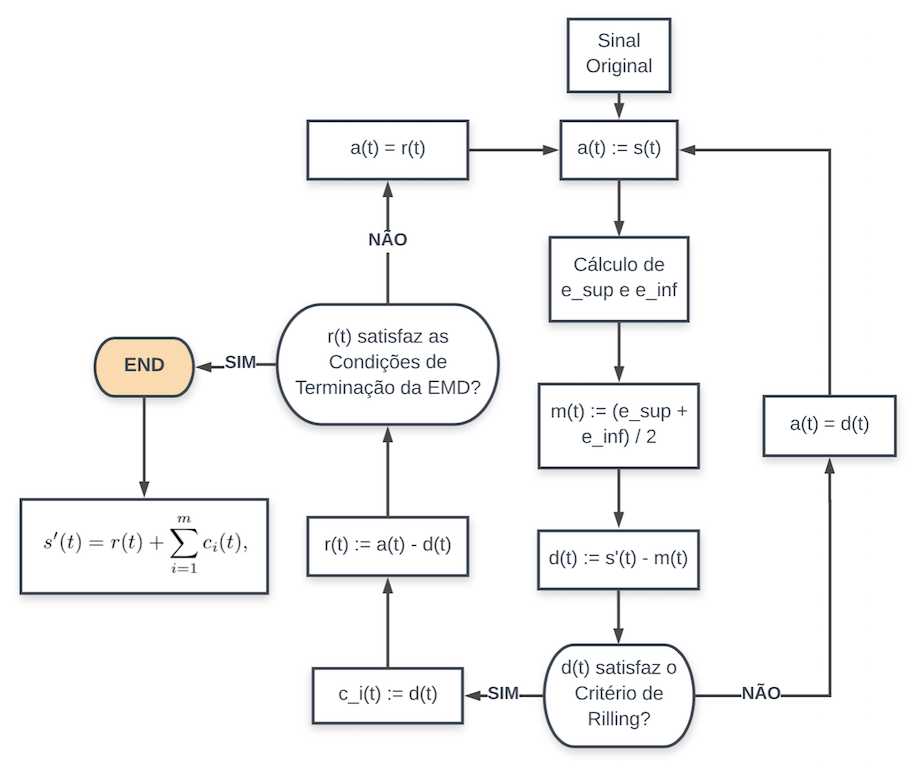
\includegraphics[width=\columnwidth]{esquema.png}
    \caption{Algoritmo para a descoberta da \textit{EMD} de um dado sinal}
    \label{fig:esquema}
\end{figure}
\end{center}

\section{Implementação}
\label{sec:implement}

\par Descreve-se agora a classe \textsc{EMD}, desenvolvida para a implementação da \textit{EMD} num dado sinal $ s(t) $. Para isto, a classe \textsc{EMD}:

\begin{enumerate}
    
    \item Agrega os sinais auxiliares $s(t)$, $e_{m, sup}(t)$, $e_{m, sup}(t)$, $m(t)$, $e_{d, sup}(t)$, $e_{d, sup}(t)$, $d(t)$ e $r(t)$ como membros privados, de tal forma que cada sinal é representado por um template \textsc{Vector< >} com argumentos da classe \textsc{Point}, onde a classe \textsc{Point} designa um par ordenado formado da forma $ \left( t, y(t) \right) $.
    
    \item Implementa um método público \texttt{FindIMFs}, que implementa o algoritmo descrito no Diagrama \ref{fig:esquema} de forma a extrair sucessivas \texttt{IMFs} do $ s(t) $. Este recorre aos métodos privados mencionados abaixo:
        
        \begin{enumerate}[label = \textbf{(\arabic*)} ]
        
            \item \texttt{SiftingProcess}, que extrai uma \textit{IMF} $ d(t) $ do sinal $ s(t) $, com recurso aos métodos, que, a cada iteração:
            
            \begin{enumerate}[label = \textbf{(\arabic*)} ]
            
                \item \texttt{SetMean}, que determina o sinal $ m(t) $. Para isso, calcula os envelopes $ e_{m, \text{sup}}(t) $ e $ e_{m, \text{inf}}(t)$, via os métodos \texttt{GetMax} e \texttt{GetMin}, para cálculo dos extremos locais, e depois os métodos \texttt{SetEMin} e \texttt{SetEMax}, para sua interpolação, utilizando a classe \textbf{SplineInterpolator}.
                
                \item \texttt{GetDetail}, que identifica o detalhe.
            
            \end{enumerate}
            
            \item O critério de terminação é implementado no método \texttt{ContinueCycle}. Para avaliar se o resíduo é aproximadamente constante, calcula-se a amplitude média do resíduo e a amplitude média do sinal inicial. Se a distancia em todos os pontos do resíduo em relação à amplitude média for inferior a $10\%$ do valor da amplitude média inicial considera-se que o resíduo é constante. Para avaliar o número de extremos utilizam-se novamente os métodos \texttt{GetMax} e \texttt{GetMin}.
        
        \end{enumerate}
        
    De notar que foram utilizadas diversas as classes desenvolvidas ao longo do semestre de forma a se poder interpolar os extremos com o Cubic Spline tais como: \textsc{EqSolver}, \textsc{FCmatrix}, \textsc{FCmatrixBanded}, \textsc{Vec}, \textsc{FCtools}, \textsc{DataPoints}. Também foi utilizada a classe desenvolvida pelos docentes \textsc{cFCGraphics} de forma a facilitar o desenho de gráficos usando a biblioteca \textsc{ROOT}.

\end{enumerate}

\section{Processo de Mirroring}

Para permitir um bom comportamento do interpolador nos extremos do intervalo é importante definir uma técnica de Mirroring, ou seja, utilizar pontos extra fora do intervalo em questão. Nos métodos \texttt{GetMax} e \texttt{GetMin} os extremos do intervalo são considerados como extremos. Como nem sempre devem ser interpolados, foi necessário criar um critério de inclusão ou não destes extremos:

\begin{enumerate}[label = \textbf{(\arabic*)} ]

\item Se o primeiro máximo for um extremo do intervalo, apenas é utilizado para a interpolação se for superior ou igual ao máximo seguinte. Se o último máximo for um extremo do intervalo, apenas é utilizado para a interpolação se for superior ou igual ao máximo anterior.

\item Se o primeiro mínimo for um extremo do intervalo, apenas é utilizado para a interpolação se for inferior ou igual ao mínimo seguinte. Se o último mínimo for um extremo do intervalo, apenas é utilizado para a interpolação se for inferior ou igual ao mínimo anterior.

\item Os valores que são espelhados são sempre o primeiro máximo ou mínimo não incluindo os extremos do intervalo.

\end{enumerate}

\begin{comment}

O algoritmo utilizado para isto apresenta-se abaixo. Note-se que $s$ e $max$ representam os valores da amplitude do sinal original e dos máximos a interpolar.

\begin{algorithm}[H]
\eIf{$max[0]$ == $s[0]$}{
    \eIf{$max[0]$ $\geqslant$ $max[1]$}{
        use $max[0]$ for interpolation
    } {
        don't use $max[0]$ for interpolation
    }
} {
    use $max[0]$ for interpolation
}
\caption{Spline on Left Side - Maxima}
\end{algorithm}

\begin{algorithm}[H]
\eIf{$max[max\_size-1]$ == $s[N-1]$}{
    \eIf{$max[max\_size-1]$ $\geqslant$ $max[max\_size-2]$}{
        use $max[max\_size-1]$ for interpolation
    } {
        don't use $max[max\_size-1]$ for interpolation
    }
} {
    use $max[max\_size-1]$ for interpolation
}
\caption{Spline on Right Side - Maxima}
\end{algorithm}

\begin{algorithm}[H]
\eIf{$min[0]$ == $s[0]$}{
    \eIf{$min[0]$ $\leqslant$ $min[1]$}{
        use $min[0]$ for interpolation
    } {
        don't use $min[0]$ for interpolation
    }
} {
    use $min[0]$ for interpolation
}
\caption{Spline on Left Side - Minima}
\end{algorithm}
	
\begin{algorithm}[H]
\eIf{$min[min\_size-1]$ == $s[N-1]$}{
    \eIf{$min[min\_size-1]$ $\leqslant$ $min[min\_size-2]$}{
        use $min[min\_size-1]$ for interpolation
    } {
        don't use $min[min\_size-1]$ for interpolation
    }
} {
    use $min[min\_size-1]$ for interpolation
}
\caption{Spline on Right Side - Minima}
\end{algorithm}

\end{comment}

\section{Exemplos de aplicação}
\label{sec:exemplos}

\subsection{Soma de senos}

\par A seguinte função foi discretizada em 400 pontos no intervalo [0,4[ para se poder utilizar o processo de \textit{EMD} para serem obtidas \textit{IMF}s.

\begin{equation*}
    s(t) = 0.5 \: \sin (1 \times 2 \pi t) + 0.8 \: \sin (3 \times 2 \pi t) +  1.5 \: \sin (5 \times 2 \pi t)
\end{equation*}

\subsubsection{Resultados e Análise}

\par Foram obtidas 3 \textit{IMF}s e os dados presentes na tabela 1.




\par Visto que o sinal original resulta da soma de três funções sinusoidais, é de esperar que o número de \textit{IMF}s seja três, tal como obtido. 
\par A frequência média de cada uma das \textit{IMF}s está de acordo com as frequências das componentes do sinal original 1, 3 e 5 Hz. Por outro lado, apenas duas das amplitudes médias estão de acordo com as esperadas visto que a amplitude média da segunda \textit{IMF} deveria ser 0.8.


\par No entanto, note-se: ao tornar 10 vezes mais rígidos os critérios para verificar se um detalhe era uma \textit{IMF}, isto é, o critério de Rilling, as amplitudes obtidas foram muito mais exatas, como mostra o espetro de Hilbert abaixo.
\par Num caso como este, um sinal artificial obtido através de uma função contínua bem conhecida, faz sentido tornar este critério mais rígido. No entanto, esta é uma modificação que foi feita conhecendo o sinal \textit{a priori}. Tornar os critérios mais rígidos desta maneira não faria sentido para analisar um sinal físico do qual não se tem nenhuma informação prévia com um método adaptável como este. Assim, foram mantidos os valores recomendados quando a aplicar o critério de Rilling. Deixe-se a nota, no entanto, que, para analisar diferentes conjuntos de dados, pode ser necessário usar critérios de paragem diferentes, tanto para acabar de encontrar \textit{IMF}s como para aceitar um detalhe como \textit{IMF}.

\begin{center}
\begin{figure}[H]
\centering
    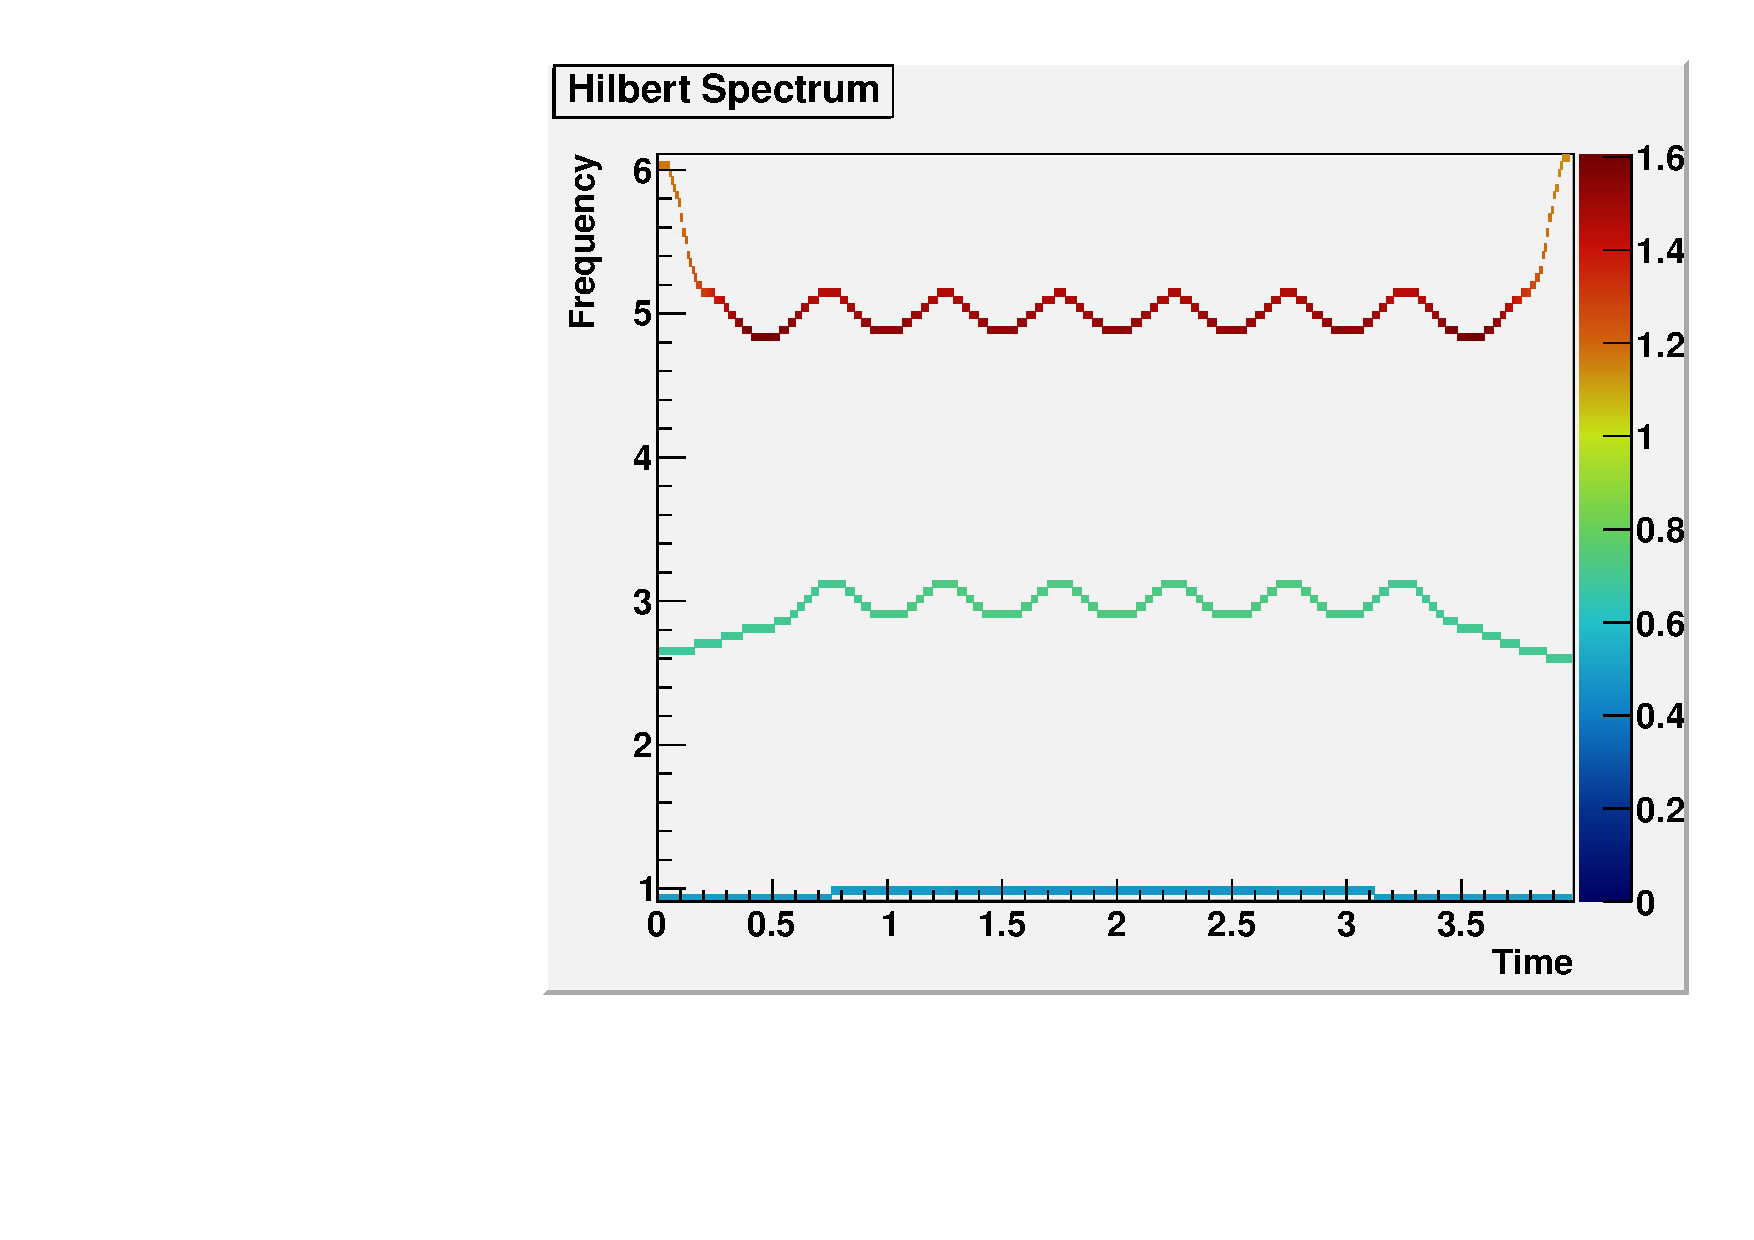
\includegraphics[width=7cm]{hilbert-more-precision.pdf}
    \caption{Espetro de Hilbert obtido com um critério de Rilling mais rígido}
\end{figure}
\end{center}

\par De acordo com os coeficientes de correlação, nota-se que a primeira \textit{IMF} é a mais significativa. A amplitude da primeira \textit{IMF} é, também, a mais elevada.
\par Abaixo encontram-se alguns gráficos relevantes obtidos.

\end{multicols}

\begin{table}[b!]
\centering
\begin{tabular}{c c c c c c}
\hline
\textbf{IMF} & \textbf{Nº de Iterações} & \textbf{Coeficiente de} & \textbf{Amplitude} & \textbf{Frequência} & \textbf{Período}\\
 &  & \textbf{Correlação} & \textbf{média} & \textbf{média} & \textbf{médio}\\
\hline
$1$ & $4$ & $0.926$ & $1.48$ & $5.06$ & $0.20$\\
$2$ & $2$ & $0.462$ & $0.42$ & $2.91$ & $0.34$\\
$3$ & $1$ & $0.325$ & $0.47$ & $0.95$ & $1.05$\\
\hline
\end{tabular}
\caption{Dados obtidos após a análise da discretização da soma de três senos}
\end{table}

\begin{multicols}{2}

%\end{multicols}

%\begin{multicols}{2}

\begin{center}
\begin{figure}[H]
\centering
    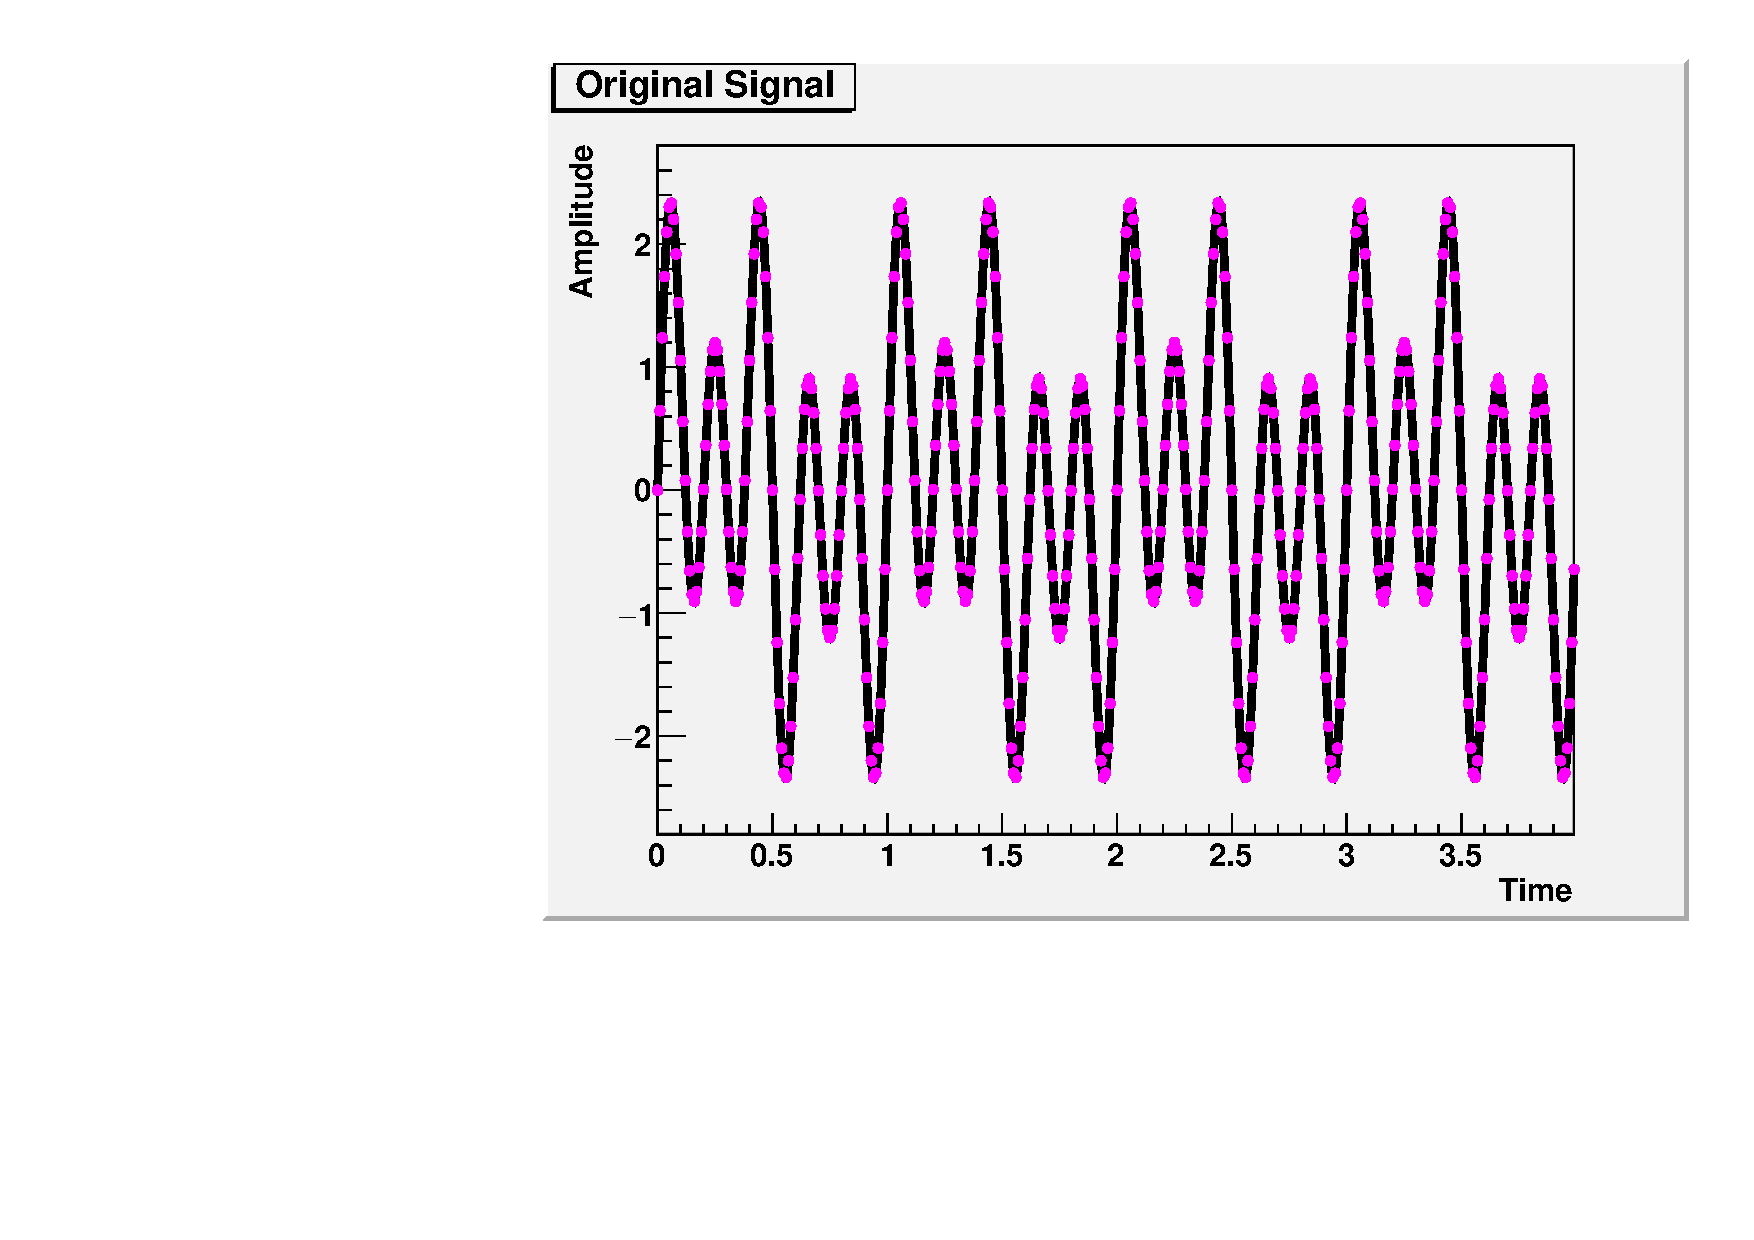
\includegraphics[width=7cm]{OriginalSignal_Sen.pdf}
    \caption{Sinal Original - Função Discreta}
\end{figure}
\end{center}

\begin{center}
\begin{figure}[H]
\centering
    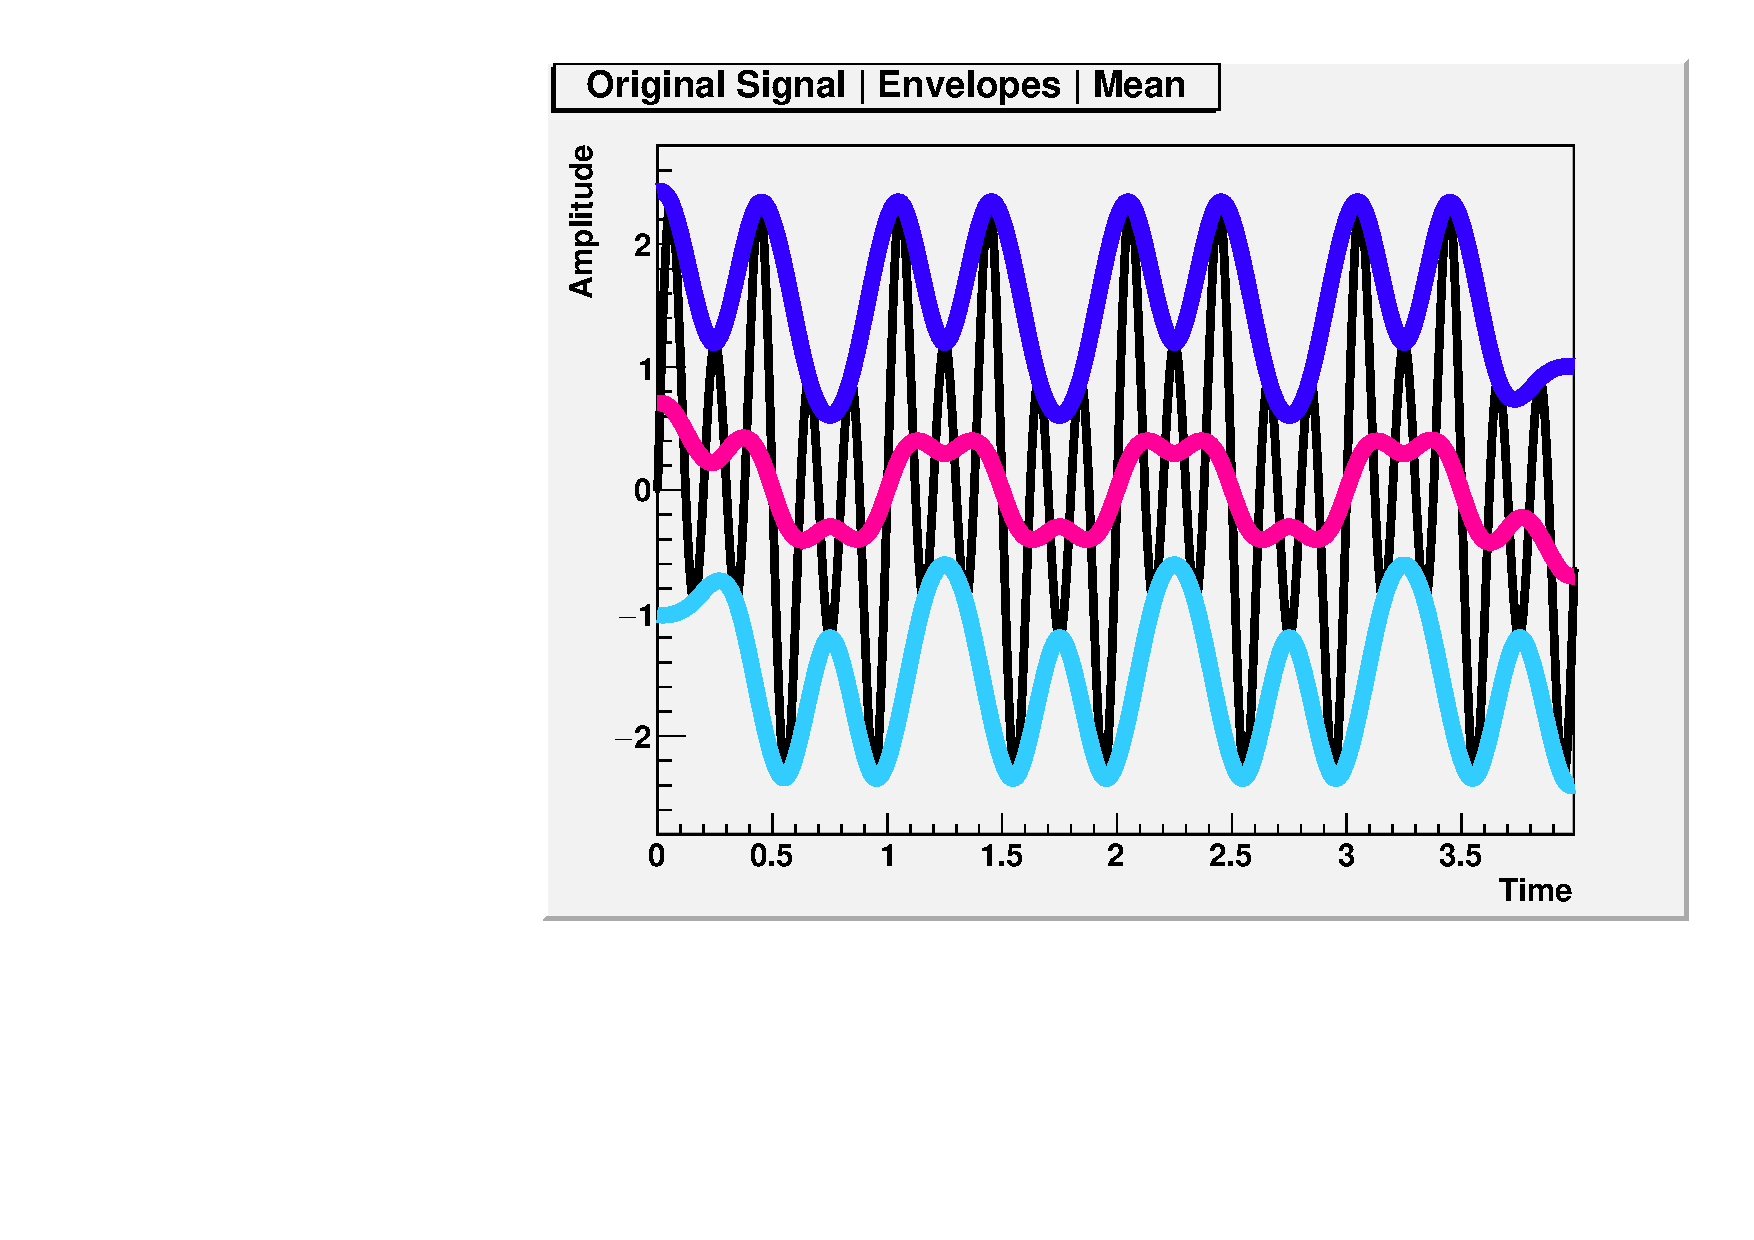
\includegraphics[width=7cm]{Signal_mean_Sen.pdf}
    \caption{Sinal Original e Respetivos Envelopes}
\end{figure}
\end{center}

\begin{center}
\begin{figure}[H]
\centering
    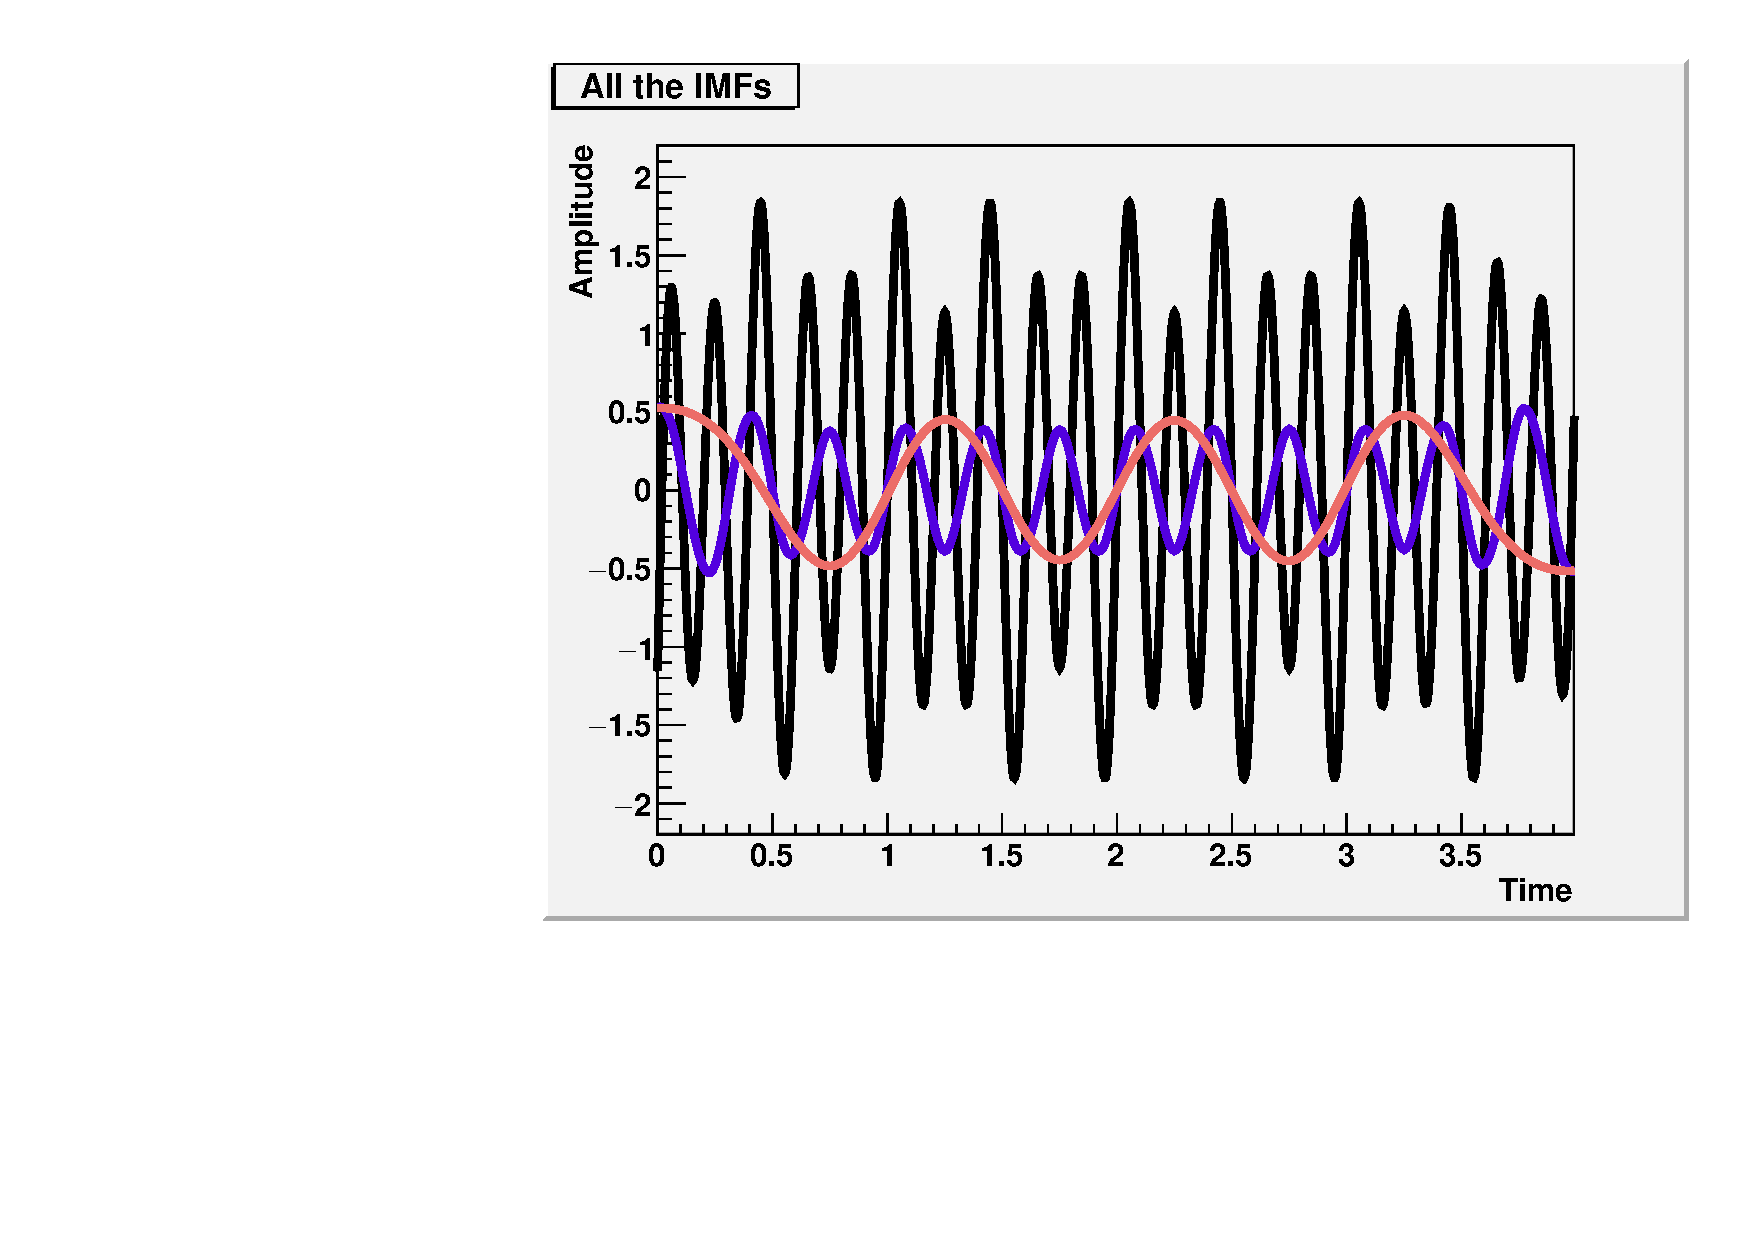
\includegraphics[width=7cm]{All_IMFs_Sen.pdf}
    \caption{IMF's - Função Discreta}
\end{figure}
\end{center}

\begin{center}
\begin{figure}[H]
\centering
    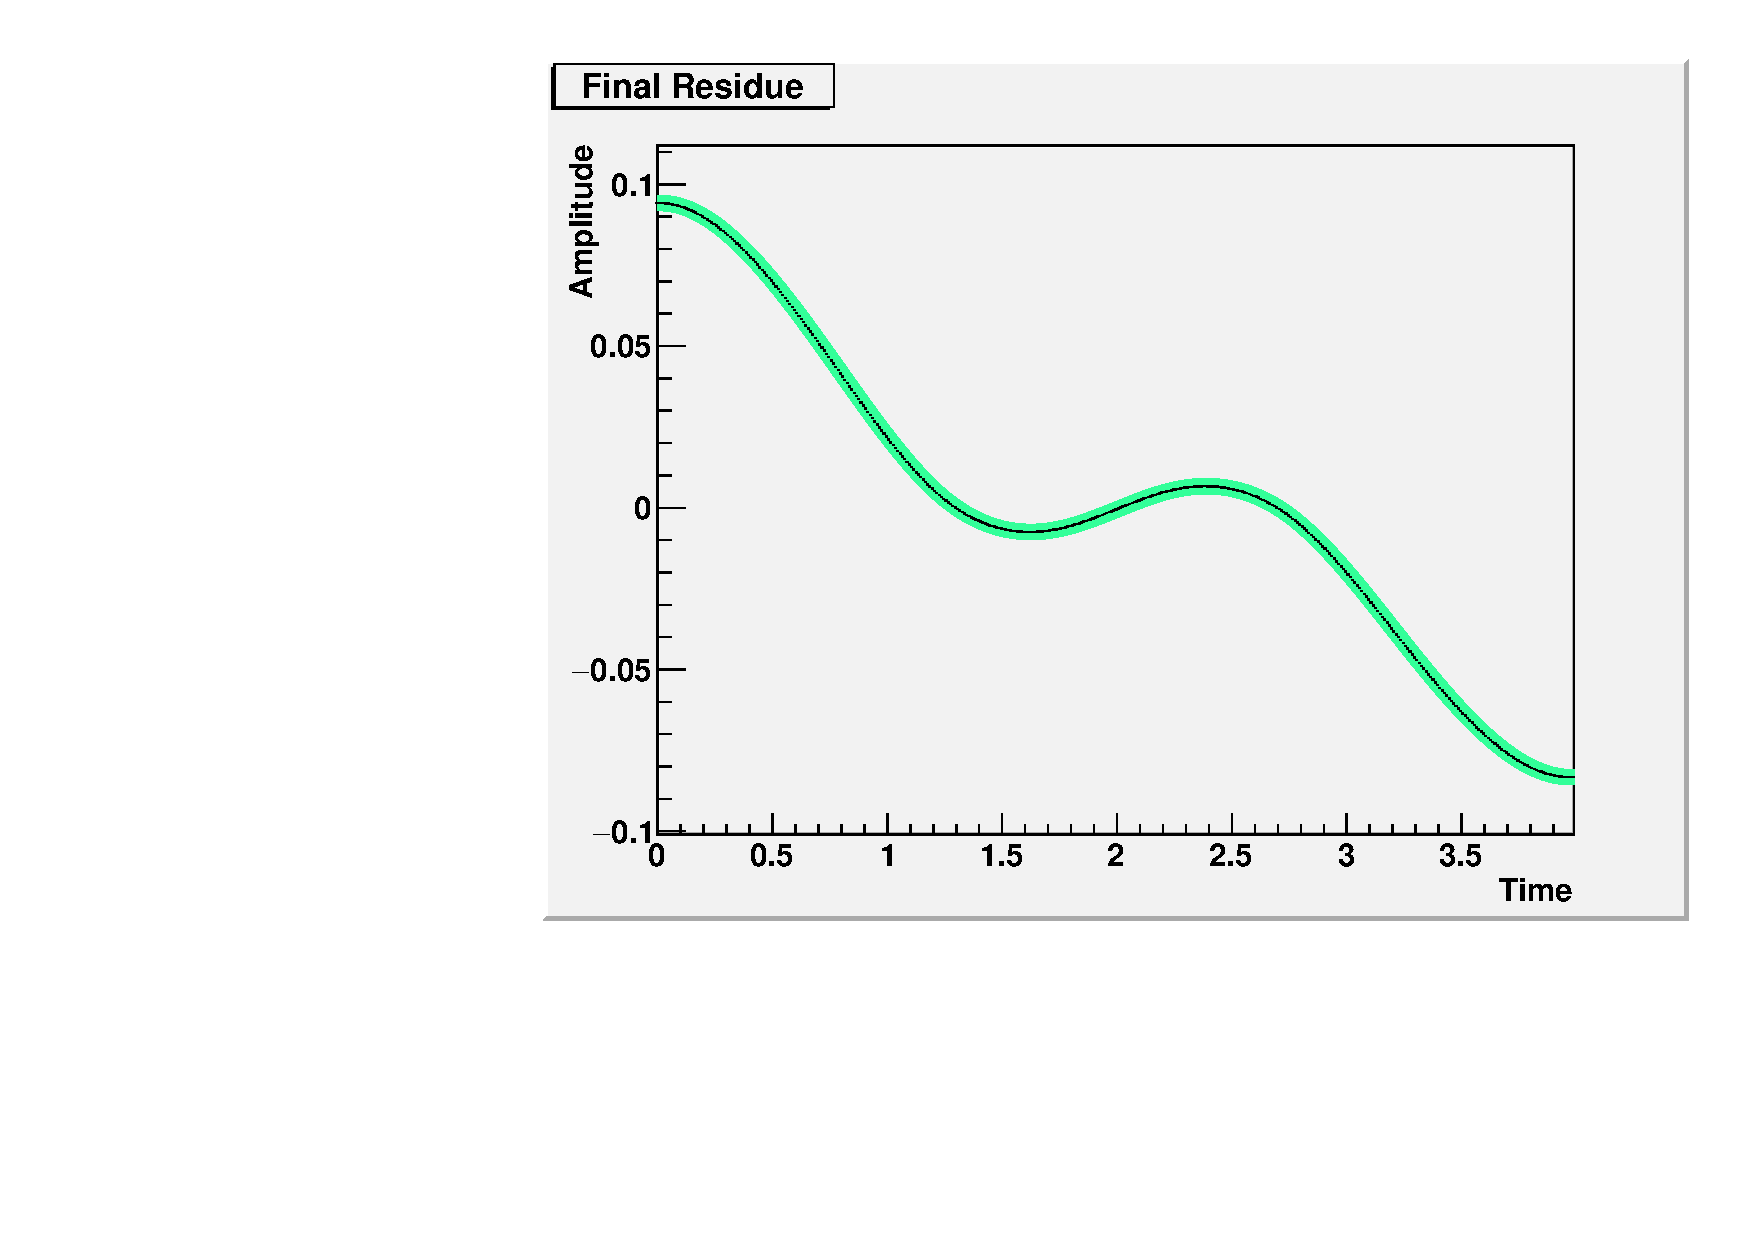
\includegraphics[width=7cm]{Residue_Sen.pdf}
    \caption{Resíduo Final - Função Discreta}
\end{figure}
\end{center}

\end{multicols}

\begin{multicols}{2}

\subsection{Número de \textit{sun spots} ao longo dos anos}

\par Depois, foi analisado o número de \textit{sun spots} (zonas da superfície do Sol - fotoesfera - com temperaturas mais baixas) desde 1749 até 2018. Foram obtidos os seguintes resultados:

\end{multicols}


\subsubsection{Resultados e Análise}

\begin{table}[H]
\centering
\begin{tabular}{c c c c c c}
\hline
\textbf{IMF} & \textbf{Nº de Iterações} & \textbf{Coeficiente de} & \textbf{Amplitude} & \textbf{Frequência} & \textbf{Período}\\
 &  & \textbf{Correlação} & \textbf{média} & \textbf{média} & \textbf{médio}\\
\hline
$1$ & $41$ & $0.13$ & $14.5$ & $4.15$ & $0.24$\\
$2$ & $34$ & $0.08$ & $12.9$ & $2.11$ & $0.47$\\
$3$ & $24$ & $0.09$ & $11.5$ & $1.13$ & $0.89$\\
$4$ & $14$ & $0.07$ & $10.9$ & $0.59$ & $1.70$\\
$5$ & $32$ & $0.28$ & $43.4$ & $0.22$ & $4.55$\\
$6$ & $6$ & $0.36$ & $51.1$ & $0.09$ & $11.11$\\
$7$ & $7$ & $0.12$ & $19.1$ & $0.04$ & $25.00$\\
$8$ & $6$ & $0.14$ & $33.3$ & $0.02$ & $50.00$\\
$9$ & $9$ & $0.15$ & $11.1$ & $0.01$ & $100.00$\\
\hline
\end{tabular}
\caption{Dados obtidos após a análise do número de \textit{sun spots} ao longo de 270 anos}
\end{table}

\begin{multicols}{2}

\begin{center}
\begin{figure}[H]
\centering
    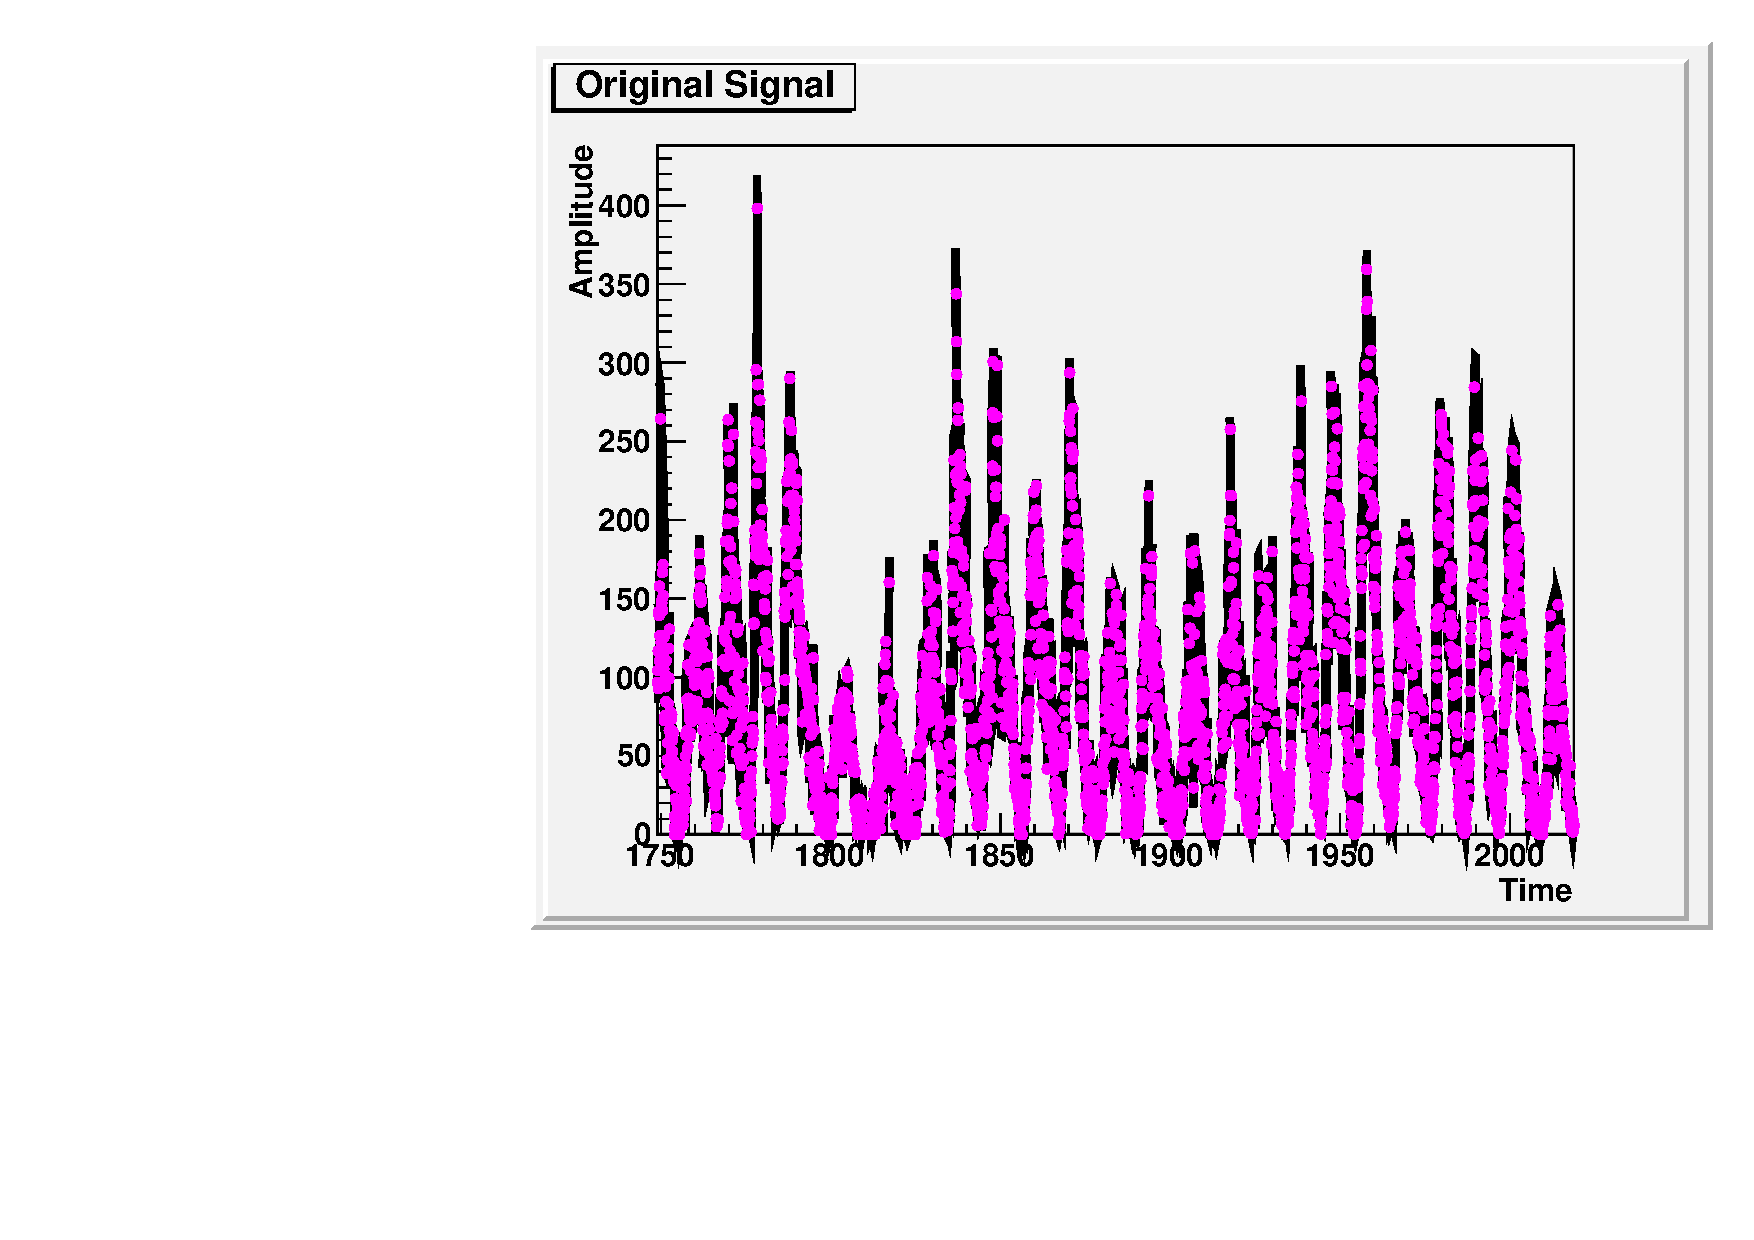
\includegraphics[width=7cm]{OriginalSignal_Sun.pdf}
    \caption{Sinal Original}
\end{figure}
\end{center}

\begin{center}
\begin{figure}[H]
\centering
    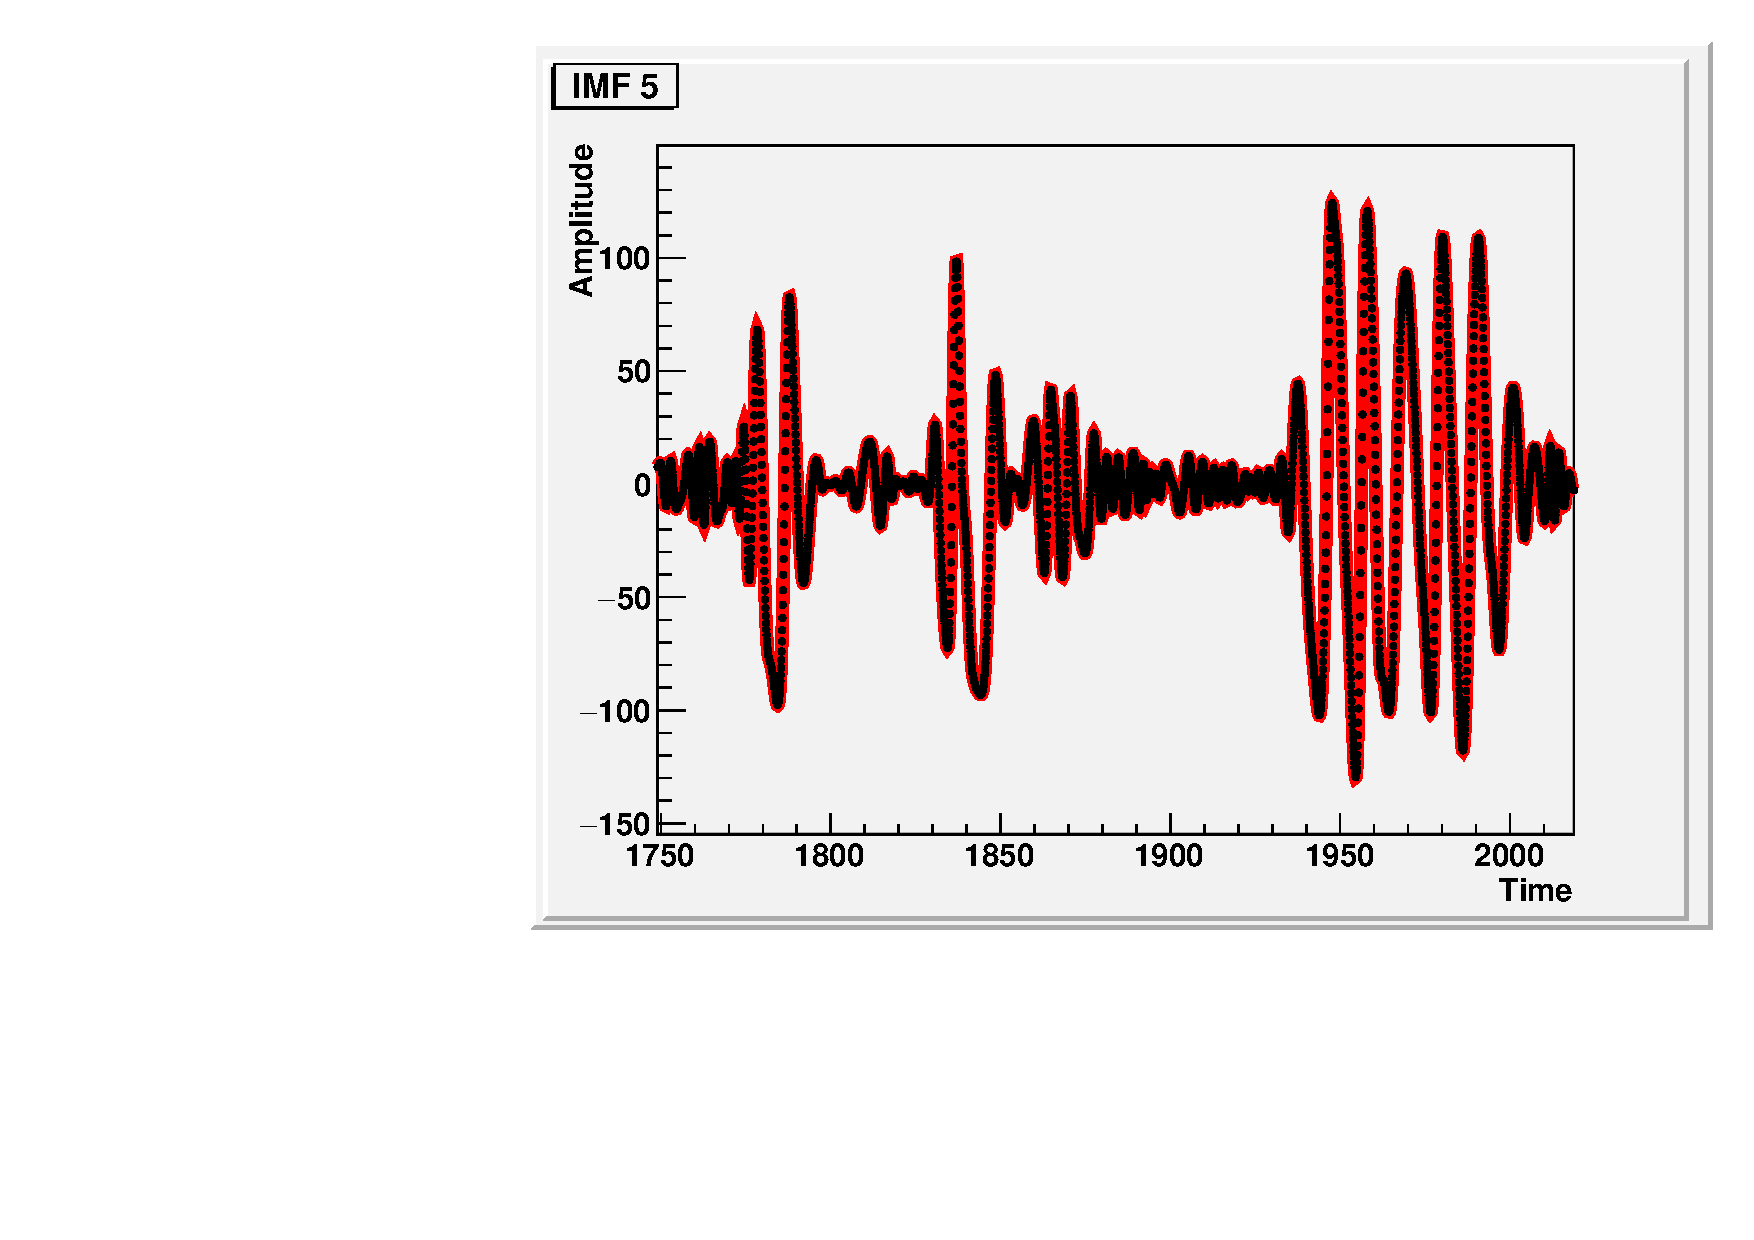
\includegraphics[width=7cm]{IMF5_Sun.pdf}
    \caption{5ª IMF}
\end{figure}
\end{center}

\begin{center}
\begin{figure}[H]
\centering
    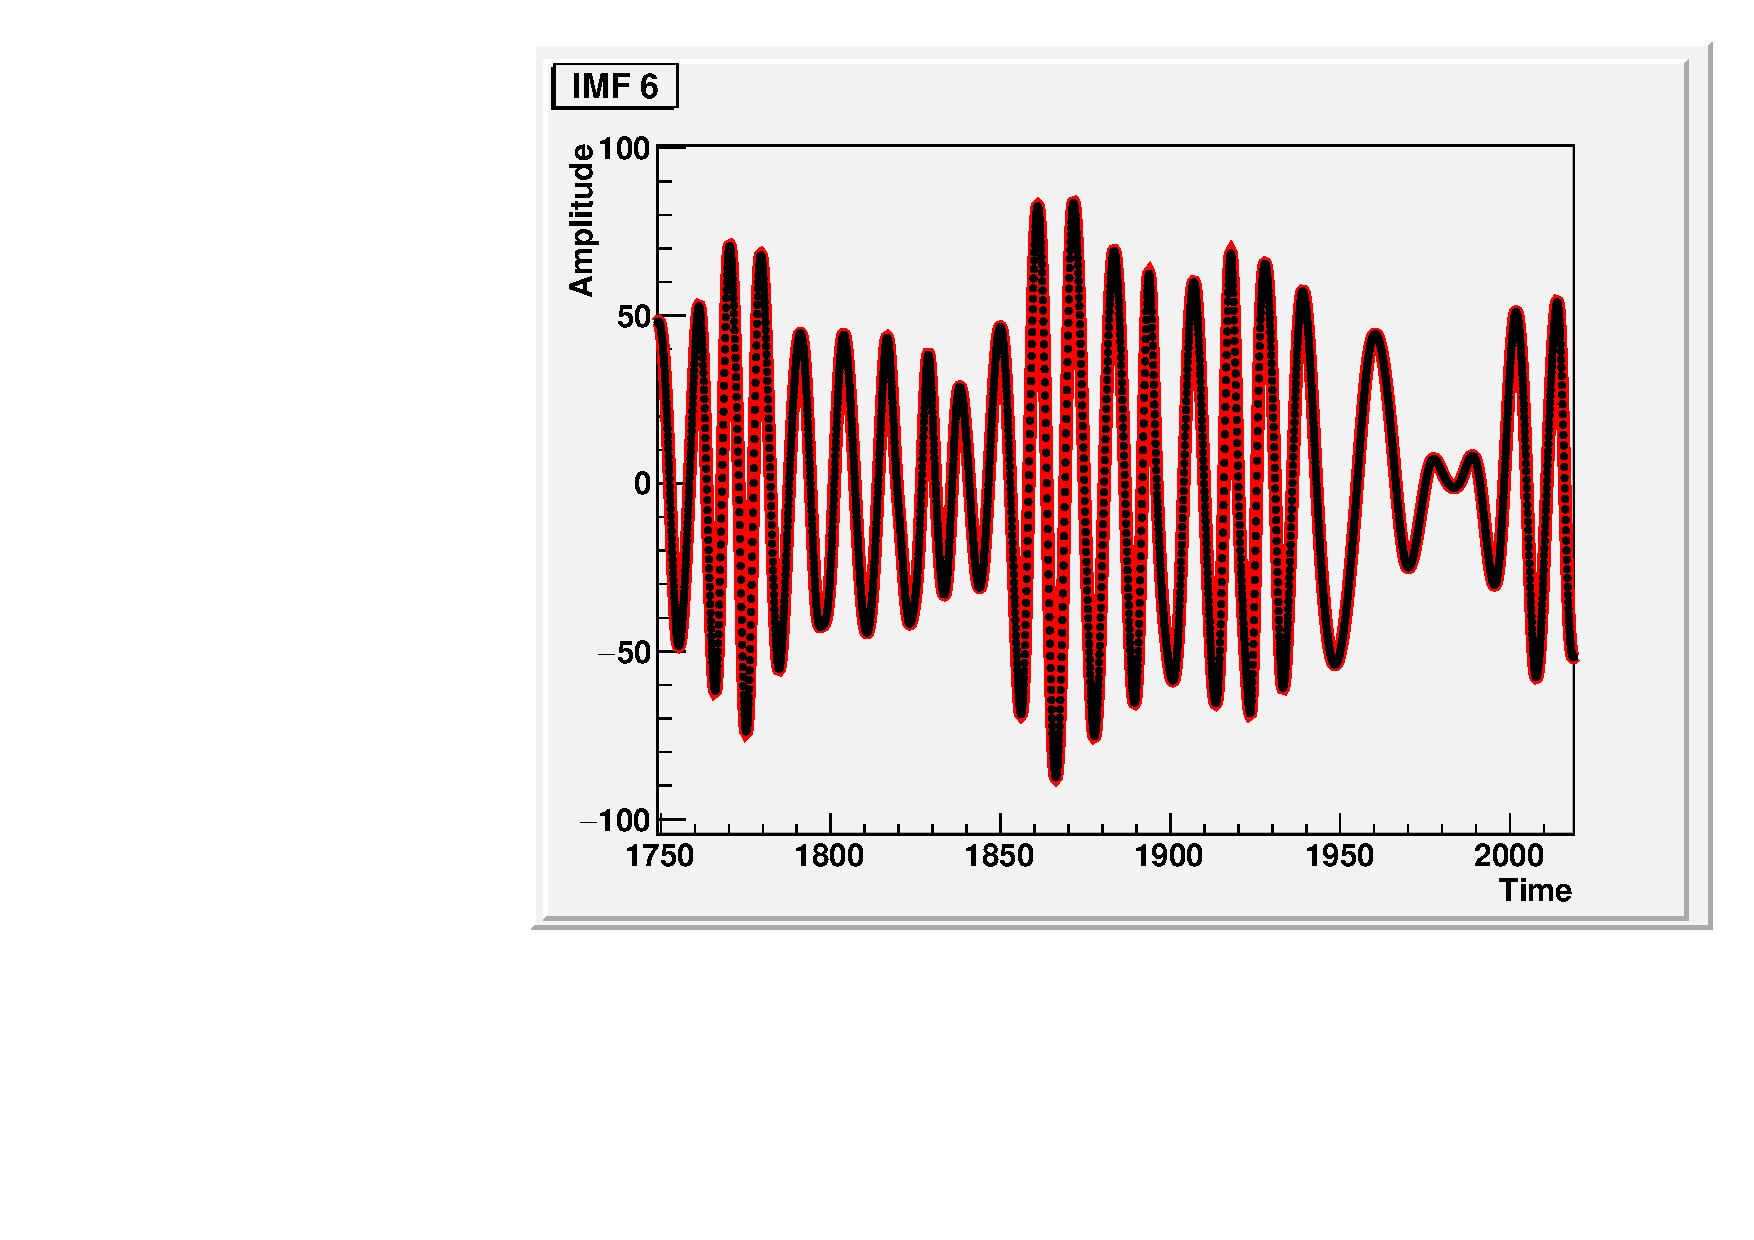
\includegraphics[width=7cm]{IMF6_Sun.pdf}
    \caption{6ª IMF}
\end{figure}
\end{center}

\begin{center}
\begin{figure}[H]
\centering
    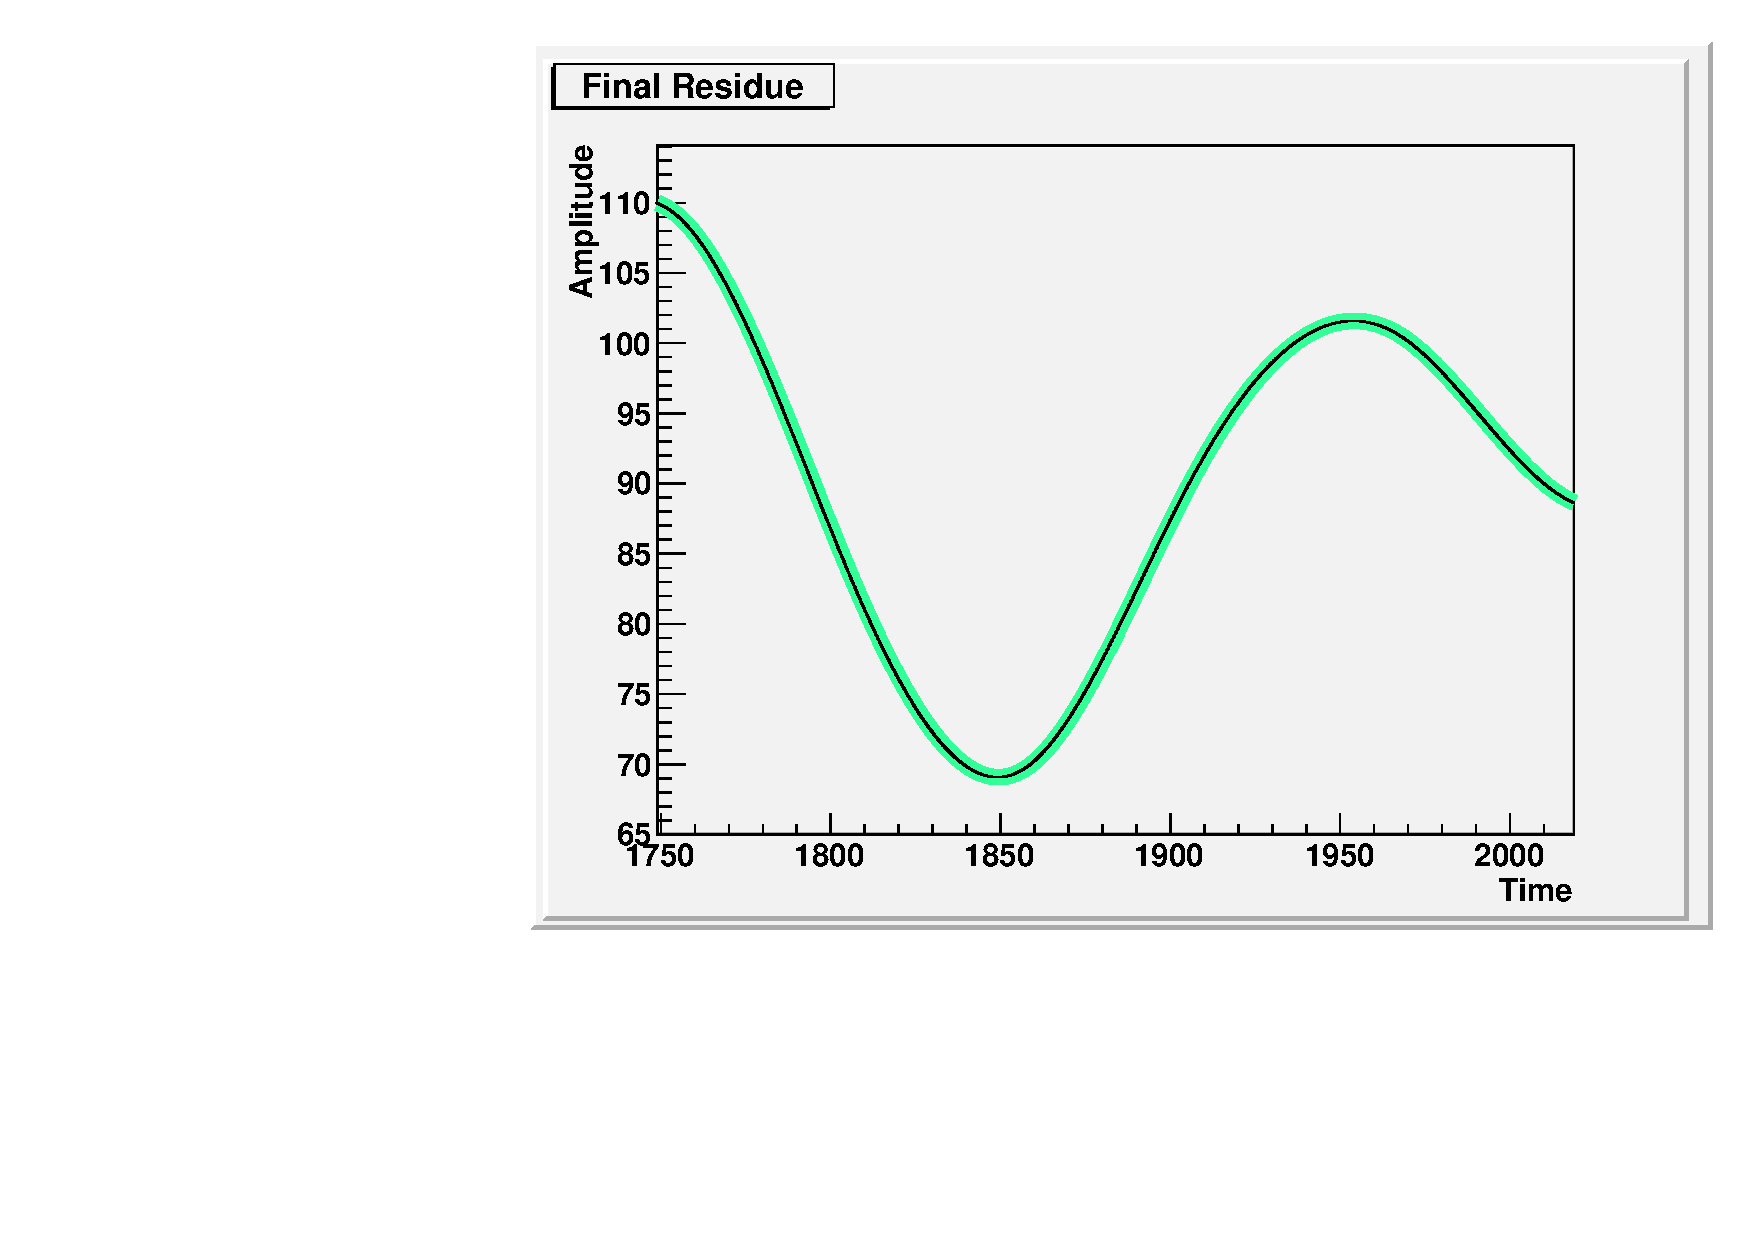
\includegraphics[width=7cm]{Residue_Sun.pdf}
    \caption{Resíduo Final - Função Discreta}
\end{figure}
\end{center}

\end{multicols}

\begin{multicols}{2}

\section{Análise Final e Conclusão}

\par Neste trabalho, pretendeu-se, primeiro, validar tanto o método de \textit{EMD} como o algoritmo implementado para o realizar e, depois, aplicar o método e o algoritmo a uma situação real com implicações físicas. A motivação específica para a realização do trabalho é a análise do número de \textit{sun spots} ao longo dos anos.

\subsection{Análise do método de \textit{EMD}}

\par Para tal, começou-se por analisar um sinal artificial proveniente da discretização de uma função contínua (a soma de três senos com ampitudes e frequências diferentes). Após a análise por \textit{EMD}, foram obtidas três \textit{IMF}s cuja soma se verificou ser aproximadamente o sinal inicial, com algumas flutuações. 

\par Note-se que a soma das \textit{IMF}s não ser aproximadamente igual ao sinal original não é algo problemático ou que desvalide o método. No primeiro caso analisado, na soma de senos, o resíduo era pouco importante, uma vez que a função oscilava em torno do zero da escala. No entanto, no caso da análise do número de \textit{sun spots} ao longo de vários anos, o resíduo vai ser relevante para comprovar a eficácia do método (ao somá-lo às \textit{IMF}s encontradas e comparar com o sinal original), uma vez que o sinal tem um \textit{offset} do zero que só se propaga para o resíduo (as \textit{IMF}s oscilam em torno do zero).

\par Após somar o resíduo final a estas três \textit{IMF}s, o resultado pareceu coincidir totalmente com o sinal original. Tal está concordante com a teoria, uma vez que o sinal original é suposto ser aproximadamente igual à soma das suas \textit{IMF}s mais o seu resíduo.

\par As frequências e as amplitudes destas três \textit{IMF}s eram aproximadamente iguais às dos senos, com algumas flutuações.

\par Concluiu-se, também, que há uma relação entre a amplitude e a significância das \textit{IMF}s: quanto maior for a amplitude da \textit{IMF}, maior será o seu coeficiente de correlação.

\par Esta primeira aplicação permite validar tanto o método como o algoritmo: é possível, de facto, decompor um sinal e obter dados significativos para o mesmo. 
O método de \textit{EMD} é rápido e de fácil implementação que obtem resultados viáveis.
\par No entanto, tal como  é verificável na apresentação de resultados, há que ter em conta que pode ser necessário ajustar os critérios de paragem aos dados do sinal. Afinal de contas, este é um método empírico.

\subsection{Análise do número de \textit{sun spots}}

\par Após verificar a validação do método, foi analisado o número de \textit{sun spots} nos últimos 270 anos. Estes \textit{sun spots} são zonas da superfície solar onde o campo magnético é muito mais forte do que em qualquer outra área do Sol. Por causa deste forte campo magnético, a temperatura daquele local diminui (o campo magnético forte inibe o fluxo de gás quente que vem do interior do Sol para a superfície). Estes locais aparecem usualmente aos pares e com polaridade magnética oposta.
\par O número destes \textit{sun spots} aumenta e diminui de acordo com um ciclo de cerca de 11 anos - o ciclo solar\footnote{Desde 1749 até 2018, houve 23 ciclos solares completos.}. Este intervalo de tempo corresponde ao tempo entre cada mudança de polaridade do campo magnético do Sol (ou seja, a mudança de polaridade tem um período médio de 22 anos).
\par Embora a razão pela qual os \textit{sun spots} existam e se comportem assim ainda está a ser investigada, parece que estes fenómenos são a consequência visível do facto de tubos de fluxo magnético presentes na zona de convecção solar (a camada solar antes da fotosfera) ficarem "enrolados" por rotação diferencial (diferentes zonas rodarem com velocidades angulares diferentes). Quando a tensão sobre os tubos chega a um certo limite, eles perfuram a superfície solar e impedem a convecção. 
\par A análise feita parece estar em concordância com o ciclo solar: a \textit{IMF} com o maior coeficiente de correlação (\textit{IMF} 6) apresenta um período médio de 11.1 anos, o que coincide com o esperado ciclo solar. A sua amplitude é também a maior (51.1). Podemos concluir, assim, que cerca de 50 \textit{sun spots} aparecem e desaparecem por ciclo solar.
\par A \textit{IMF} número 5 (com o segundo maior coeficiente de correlação) apresenta um período médio de cerca de 5 anos, aproximadamente metade do ciclo solar, e tem uma amplitude média de cerca de 43 \textit{sun spots}. Pode-se concluir, assim, que o número de \textit{sun spots} oscila, também, com metade do ciclo solar. 
\par As \textit{IMF}s número 1,2,3 e 4, dado o seu muito baixo coeficiente de correlação e alta frequência, podem ser consideradas como irrelevantes para a análise do número de sunspots e ser consideradas ruído.
\par As \textit{IMF}s número 7,8 e 9 têm um coeficiente de correlação também baixo mas podem ter algum significado físico relevante. Aliás, uma vez que o campo magnético do sol muda de polaridade a cada 22 anos, faz sentido que uma das \textit{IMF}s tenha um período médio de 25 anos, mesmo que a sua amplitude seja de apenas 19 \textit{sun spots}. A \textit{IMF} número 8 tem uma amplitude já mais elevada (33.3) e um período médio de 50 anos.
\par Note-se também que o resíduo após o processo de \textit{EMD}\footnote{O resíduo final mostra a tendência dos dados.} mostra os dois períodos com o menor e o maior número de \textit{sun spots} neste período de tempo: o chamado mínimo de Dalton (1790-1820) e o chamado máximo moderno (1900-presente).

\begin{thebibliography}{9}
\bibitem{lamport94}
 Barão, F., Coelho, R., Orcinha, M., Couto, C., Dpt. de Física, IST,
 acedido a 31 de Dezembro de 2018, $<$\textit{http://labrc.ist.utl.pt/ComputPhys.web/Projecto/P.html}$>$
\bibitem{lamport94}
 WDC-SILSO, Observatório Real da Bélgica, Bruxelas,
 acedido a 25 de Dezembro de 2018, 
 $<$\textit{http://www.sidc.be/silso/datafiles}$>$
\bibitem{lamport94}
 \textit{National Weather Service}, Sioux Falls, SD, EUA,
 acedido a 31 de Dezembro de 2018, 
 $<$\textit{https://www.weather.gov/fsd/sunspots}$>$
\end{thebibliography}

\end{multicols}

\section{Anexos}

\begin{center}
\begin{figure}[H]
\centering
    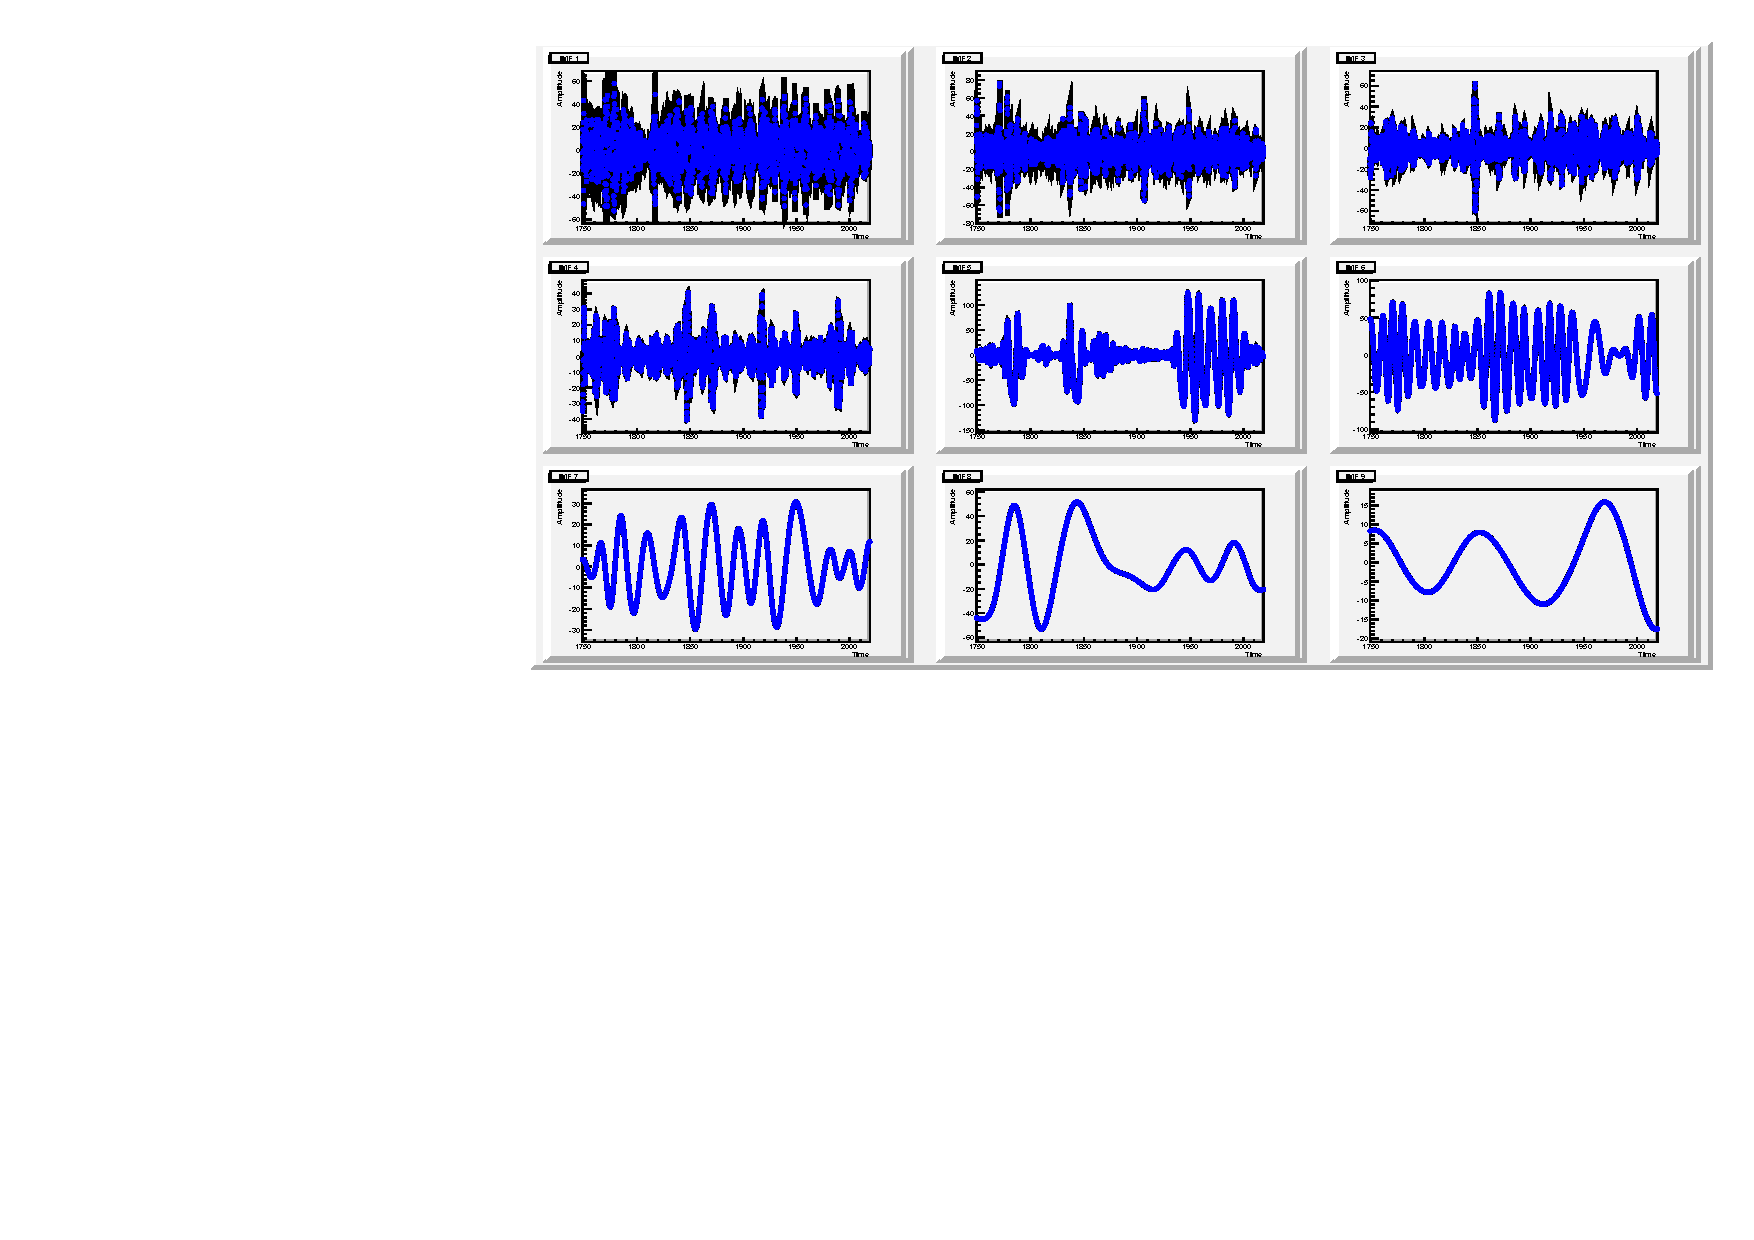
\includegraphics[width=\columnwidth]{IMFs_Sun.pdf}
    \caption{IMF's do segundo exemplo}
\end{figure}
\end{center}

\end{document}